\section{Sp\-Turbulence\-Op.h File Reference}
\label{SpTurbulenceOp_8h}\index{SpTurbulenceOp.h@{SpTurbulenceOp.h}}
{\tt \#include \char`\"{}Sp\-Grid.h\char`\"{}}\par
{\tt \#include \char`\"{}Sp\-Stream\-Operator.h\char`\"{}}\par
{\tt \#include \char`\"{}Sp\-Stream\-Buffer.h\char`\"{}}\par
{\tt \#include \char`\"{}Sp\-Stream\-Basis.h\char`\"{}}\par
{\tt \#include \char`\"{}Sp\-Gpu\-Program.h\char`\"{}}\par
{\tt \#include \char`\"{}Sp\-Stream\-Feedback.h\char`\"{}}\par
{\tt \#include \char`\"{}Sp\-Sp\-Glsl\-Vertex\-Program.h\char`\"{}}\par
{\tt \#include \char`\"{}Sp\-Glsl\-Fragment\-Program.h\char`\"{}}\par


Include dependency graph for Sp\-Turbulence\-Op.h:\begin{figure}[H]
\begin{center}
\leavevmode
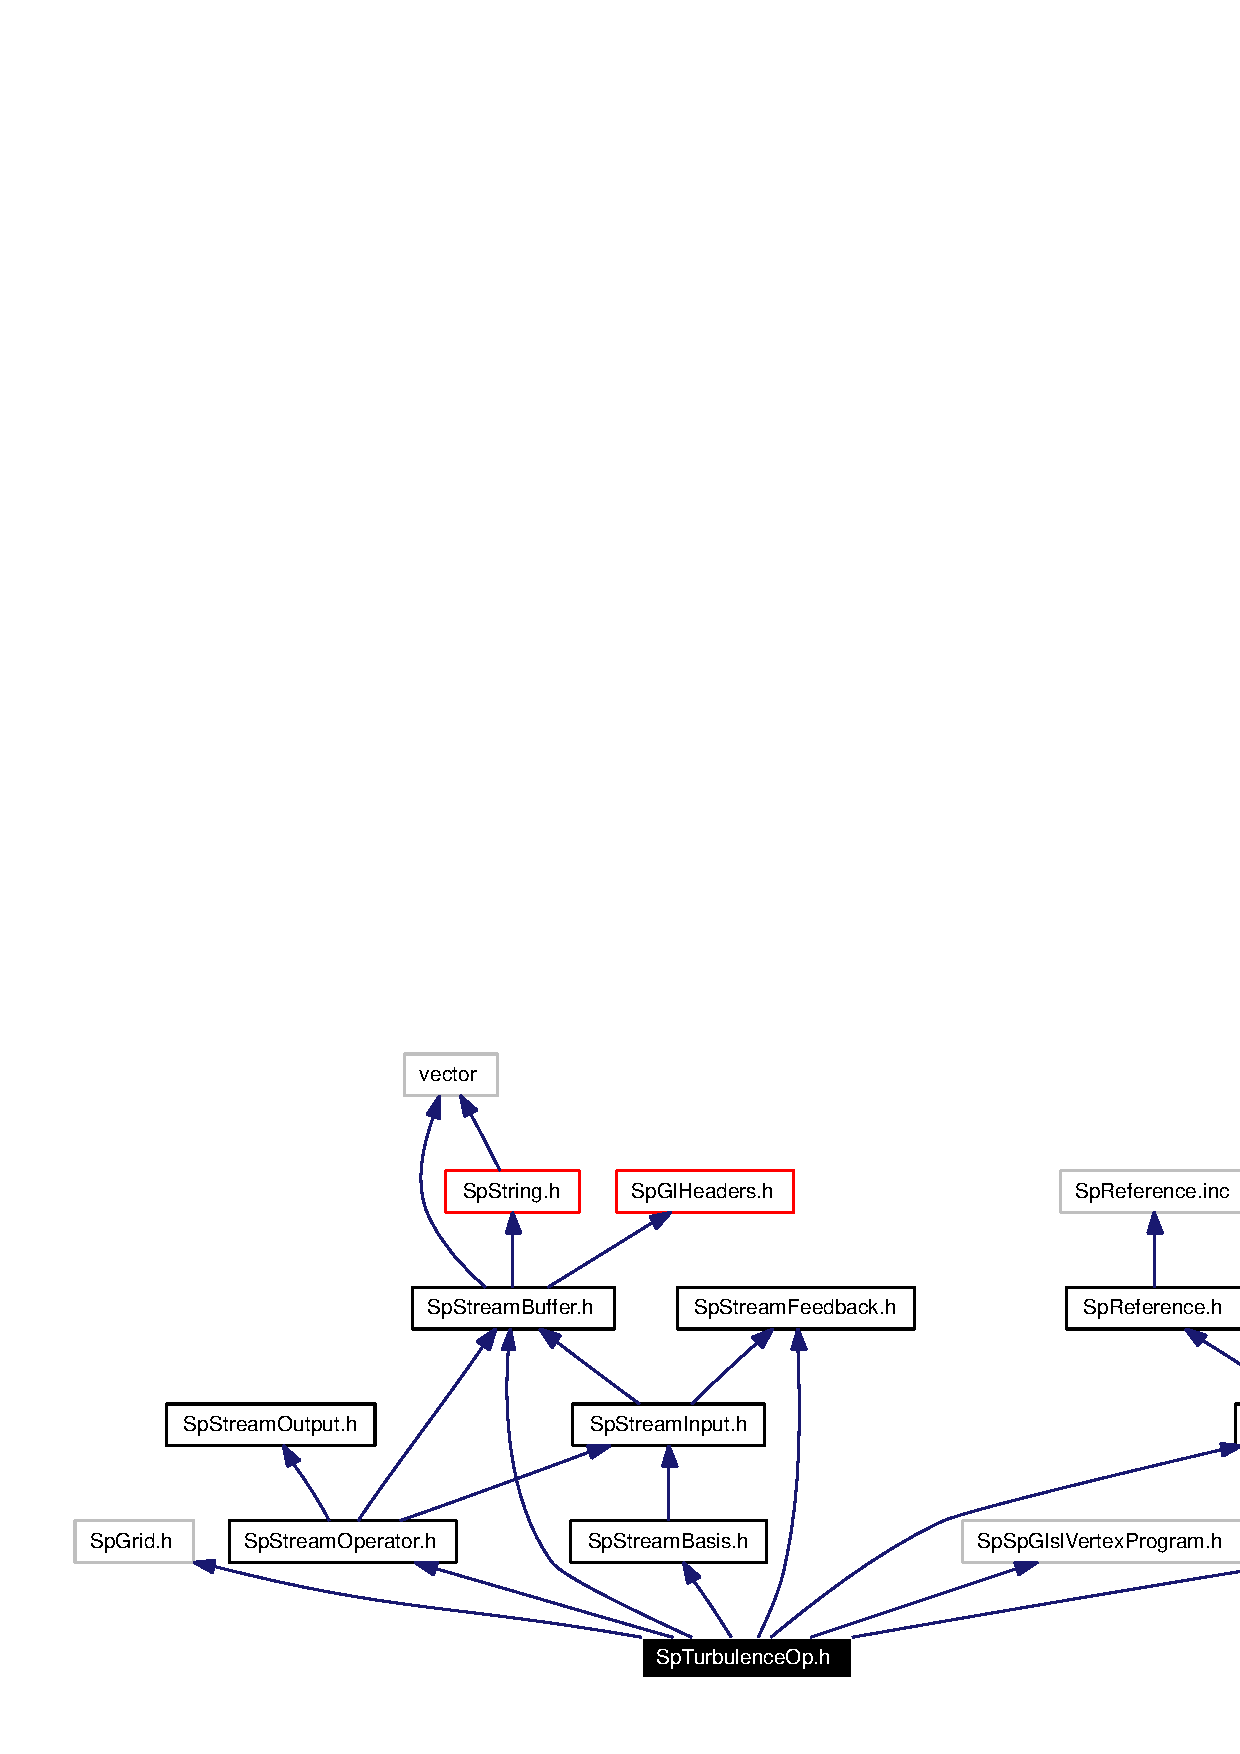
\includegraphics[width=393pt]{SpTurbulenceOp_8h__incl}
\end{center}
\end{figure}


This graph shows which files directly or indirectly include this file:\begin{figure}[H]
\begin{center}
\leavevmode
\includegraphics[width=73pt]{SpTurbulenceOp_8h__dep__incl}
\end{center}
\end{figure}
\subsection*{Namespaces}
\begin{CompactItemize}
\item 
namespace {\bf Spark}
\end{CompactItemize}
\subsection*{Classes}
\begin{CompactItemize}
\item 
class {\bf Spark::Sp\-Turbulence\-Op}
\begin{CompactList}\small\item\em Turbulence stream operator to be used with a stream basis class. \item\end{CompactList}\end{CompactItemize}
